%% LyX 2.0.0 created this file.  For more info, see http://www.lyx.org/.
%% Do not edit unless you really know what you are doing.
\documentclass[10pt,a4paper,oneside,english,pdfauthor=(OmarAwile),pdftitle=(PPM UserGuide)]{memoir}
\usepackage[T1]{fontenc}
\usepackage[latin9]{inputenc}
\usepackage{listings}
\setcounter{secnumdepth}{3}
\setcounter{tocdepth}{3}
\usepackage{amsmath}
\usepackage{amssymb}
\usepackage{graphicx}

\makeatletter

%%%%%%%%%%%%%%%%%%%%%%%%%%%%%% LyX specific LaTeX commands.
\special{papersize=\the\paperwidth,\the\paperheight}


%%%%%%%%%%%%%%%%%%%%%%%%%%%%%% Textclass specific LaTeX commands.
\numberwithin{figure}{section}
\numberwithin{equation}{section}
\newenvironment{lyxlist}[1]
{\begin{list}{}
{\settowidth{\labelwidth}{#1}
 \setlength{\leftmargin}{\labelwidth}
 \addtolength{\leftmargin}{\labelsep}
 \renewcommand{\makelabel}[1]{##1\hfil}}}
{\end{list}}

%%%%%%%%%%%%%%%%%%%%%%%%%%%%%% User specified LaTeX commands.
%\usepackage[latin1]{inputenc}
\usepackage{amsthm}
\usepackage{placeins}
\usepackage{algorithmic}
\usepackage{listings}
\usepackage{courier}
 \lstset{
         basicstyle=\small\ttfamily, % Standardschrift
         %basicstyle=\footnotesize\ttfamily, % Standardschrift
         %numbers=left,               % Ort der Zeilennummern
         numberstyle=\tiny,          % Stil der Zeilennummern
         %stepnumber=2,               % Abstand zwischen den Zeilennummern
         numbersep=5pt,              % Abstand der Nummern zum Text
         tabsize=2,                  % Groesse von Tabs
         extendedchars=true,         %
         breaklines=true            % Zeilen werden Umgebrochen
 %        keywordstyle=[1]\textbf,    % Stil der Keywords
 %        keywordstyle=[2]\textbf,    %
 %        keywordstyle=[3]\textbf,    %
 %        keywordstyle=[4]\textbf,   \sqrt{\sqrt{}} %
%         stringstyle=\color{white}\ttfamily, % Farbe der String
%         showspaces=false,           % Leerzeichen anzeigen ?
%         showtabs=false,             % Tabs anzeigen ?
%         xleftmargin=17pt,
%         framexleftmargin=17pt,
%         framexrightmargin=5pt,
%         framexbottommargin=4pt,
         %backgroundcolor=\color{lightgray},
%         showstringspaces=false      % Leerzeichen in Strings anzeigen ?        
 }
\lstloadlanguages{% Check Dokumentation for further languages ...
         %[Visual]Basic
         %Pascal
         %C
         %C++
         %XML
         %HTML
        % Java
        [95]Fortran
 }
%opening
\makeatother
\chapterstyle{southall}
\usepackage{babel}

\makeatother

\usepackage{babel}
\begin{document}

\title{PPM User's guide}

\maketitle
\tableofcontents{}


\chapter{Introduction}

The PPM library \cite{Sbalzarini:2006b,Sbalzarini:2006c} defines
the state of the art in middleware for distributed-memory particle-mesh
simulations. It hides MPI from the application programmer by introducing
an additional, transparent layer beneath the user's simulation programs
(called {}``PPM clients''). Since PPM reduces the knowledge gap,
the resulting simulations often outperform hand-parallelized codes
\cite{Sbalzarini:2006b,Sbalzarini:2010}. The PPM library is independent
of specific applications, provided the simulation is phrased in terms
of particles, meshes, or a combination of the two. PPM implements
modules for adaptive domain decomposition, communication through halo
layers, load balancing, particle-mesh interpolation, and communication
scheduling. All of this is done transparently without participation
of the user program. 

Recently PPM has undergone some major design changes: 
\begin{itemize}
\item The PPM library has been split up into two libraries. The first part
is PPM core, which provides the core parallel framework consisting
of abstractions for topologies, mappings, particles and meshes. The
second part is PPM numerics. This new library provides all the numerical
methods that were implemented based on the PPM abstractions. In this
tutorial we shall concentrate on PPM core. 
\item Using the PPM core library has been greatly simplified. The number
of arguments that must be passed to PPM routines has been reduced,
topologies are now handled internally by the library. 
\item We spent some time reorganizing the code and generating an API reference. 
\item Installing PPM has become much simpler, thanks to the use of GNU Autoconf
and Automake. 
\end{itemize}

\chapter{Obtaining and installing PPM}

PPM is distributed in source packages for the user to compile and
setup on his environment. We do not offer any pre-built packages.
Go to \texttt{}~\linebreak{}
\texttt{http://www.ppm-library.org} to download the latest version
of PPM core from the {}``Downloads'' section. PPM has been tested
with Mac OS X 10.5/10.6, Ubuntu Linux (x86-64) and Gentoo Linux (x86-64).
It should however work on any Unix system, provided all dependencies
are present and installed. In essence PPM requires following packages
to be installed: 
\begin{itemize}
\item A FORTRAN 95 compiler. For systems with Intel CPUs we recommend the
latest Intel Fortran compiler (v. 11.x). You can also use GCC's \texttt{gfortran}.
Many high-performance clusters provide also vendor-specific compilers
(e.g. IBM XL Fortran, Sun studio Fortran, NEC Fortran compiler). 
\item An MPI library. We have tested PPM with several versions of OpenMPI,
but any MPI-2 compliant library should work. It is important to compile
PPM with the same Fortran compiler as the MPI library. PPM can be
also compiled without MPI support. 
\item The METIS library. METIS is a library for graph partitioning and fill-reducing
matrix ordering. You can either download it from\\
 \texttt{http://glaros.dtc.umn.edu/gkhome/metis/metis/download} or
from the PPM website along with the PPM core source package. 
\item The \texttt{make} command and functioning shell. To build PPM we make
use of Makefiles that are interpreted by \texttt{make}. Along with
the compilers the environment where PPM core will be compiled has
to provide the standard unix shell tools and make. 
\end{itemize}
After you have downloaded the PPM core \texttt{.tar.gz} source archive
to your system and prepared the requirements you must unpack, configure
and compile the code. In the following snipped we assume you are using
OpenMPI. Please issue the \texttt{./configure -{}-help} command to
find out about how to customize PPM core: 

\begin{lstlisting}[breaklines=true,language=bash]
tar xzvpf ppmcore1.2.tar.gz cd libppm 
./configure --enable-mpi=openmpi --enable-linux --prefix=/where/ppm/shall/be/installed LDFLAGS=-L/directory/to/metis/lib
\end{lstlisting}
 Note: For most standard installations it is not necessary to specify
the compiler, as the install scripts will try to find them automatically.

the \texttt{-{}-prefix} argument requires the given directory to be
already created, otherwise the build process will fail.

If you have correctly installed all PPM dependencies and specified
the correct paths in the above command the configuration process should
exit after generating the Makefile: 
\begin{lstlisting}[language=bash]
configure: creating ./config.status 
config.status: creating Makefile
\end{lstlisting}


The next step is to compile PPM.


\section{Development}

For development and debugging, configure can be called with the --enable-dev
and the --enable-debug flags respectively.


\chapter{Understanding the PPM parallelism}

TODO: It would be useful to have a summary of what PPM actually does
and how it does it. What are the different abstractions and how are
they organized. Some diagrams/sketches would probably help a lot...

For now, the reader is referred to the seminal papers \cite{Sbalzarini:2006b,Sbalzarini:2010}.


\chapter{Sample PPM Client Application}

PPM offers a rich functionality for parallelizing the computations
that can be used in PPM clients by calling the respective subroutines.
A {}``skeleton'' of a typical PPM client consists of the following
steps: 
\begin{enumerate}
\item Read program configuration from a control file 
\item Initialize the PPM library 
\item Create the topology and fill it in with particles :

\begin{enumerate}
\item Perform the domain decomposition 
\item Generate particles 
\item Map the particles onto the topology 
\end{enumerate}
\item Initialize the ODE module and create an ODE mode 
\item Enter the main cycle of the client :

\begin{enumerate}
\item Communicate the particles on ghost layers between all processes 
\item Build neighbor lists only taking into account particles lying within
cut-off range 
\item Performing main calculations:

\begin{itemize}
\item Calculate approximations of the time derivatives using the ODE solver
\emph{or}
\item Perform particle--particle interactions 
\end{itemize}
\item Calculate other quantities using the results of previous step 
\item Update positions of individual particles 
\end{enumerate}
\item Output the results 
\item Finalize the PPM Library 
\end{enumerate}
The first step is done by means of a simple subroutine, which reads
the control file and extracts the parameter values and program configuration.
The default control file has the following format: each non-blank
line, except those that begin with a \texttt{'\#'} character, is considered
as significant and containing a pair of parameter name and value.
A sample control file is given below: \texttt{}
\begin{lstlisting}[language=bash]
#----------------------------------------------------------
# Sample control file 
#
# This line is a comment
#----------------------------------------------------------
<parameter_name> = <parameter_value> 
...
\end{lstlisting}


The second step is done by calling the \texttt{ppm\_init} subroutine.
To open the log unit a subsequent call to \texttt{ppm\_io\_set\_unit}
is required.

The topology is created using \texttt{ppm\_mktopo} subroutine, which
is the topology creation routine for particles. It performs the decomposition
of the physical space based on the position of the particles and returns
the topology id to the calling program. The subdomains are mapped
onto the processors and a neighbour list is created. The topology
itself can be obtained by subsequent call to \texttt{ppm\_topo\_get}
with the topology id as the first parameter and a pointer to the topology
itself. This allows access and modify the fields of the topology structure
directly, however, usually there is no need to do so as \texttt{ppm\_mktopo}
and other library functions should provide all the necessary functionality
for that.

The next step to perform is to fill this geometry with particles,
which is problem-specific and may be done in a variety of ways.

The mapping the particles onto topology is performed in several steps.
First \texttt{ppm\_map\_part\_global} maps the particles onto the
given topology using a global mapping (i.e. every processor communicates
with every other). Then a call to \texttt{ppm\_map\_part\_push} would
push the any relevant particle data onto the send buffer that is communicated
to the other processes via \texttt{ppm\_map\_part\_send}. Other processes
can access this data by subsequent calls to \texttt{ppm\_map\_part\_pop},
which would return the particle data (positions, strength, etc) in
the order it was put into the buffer.

It should be stressed out that if no geometric decomposition of the
domain is required, the two previous steps should be skipped.

Problems that are solved by using PPM are ususally governed by a set
of ODEs. For example, a typical transport problem of the form 
\begin{align}
\frac{Df}{Dt}=\frac{\partial f}{\partial t}+\nabla\cdot\left(\mathbf{u}f\right) & =\mathcal{L}\left(f\right),\label{eq:transport equation}
\end{align}
 leads to the system of ODEs for the positions $\mathbf{x}_{p}$,
strengths $\omega_{p}$, and volumes $v_{p}$ of the particles:

\begin{align}
\frac{d\mathbf{x}_{p}}{dt} & =\mathbf{u}_{p}\left(t\right)\label{eq:System of ODEs}\\
\frac{d\omega_{p}}{dt} & =v_{p}\mathcal{L}\left(f\right)(\mathbf{x}_{p})+\frac{dv_{p}}{dt}f\left(x_{p}\right)\nonumber \\
\frac{dv_{p}}{dt} & =v_{p}\nabla\cdot\mathbf{u}\nonumber 
\end{align}
 with $\omega_{p}=v_{p}f\left(\mathbf{x}_{p}\right)$. The differential
operator $\mathcal{L}$ can be, e.g. a diffusion operator.

To faciliate the matter, PPM library provides subroutines that give
the necessary functionality: 
\begin{itemize}
\item \texttt{ppm\_ode\_init(topo\_id,info)} -- initializes the ode solver
variable and registers the ID of the topology to be used for the ODE
solver 
\item \texttt{ppm\_ode\_create\_ode}, which creates an ODE solver for the
given integration scheme, kick-off scheme and sets whether the solver
is adaptive, 
\item \texttt{ppm\_ode\_start} -- should be called before the first step
of numerical integration. It check whether all solvers are ready then
sets them into kick-off state thus allowing the numerical integration
to begin, 
\item \texttt{ppm\_ode\_step} is the very heart of ODE solver. This routine
implements Euler, Runge-Kutta 2 and Runge-Kutta 4 numerical intgration
schemes. It should be called inside the main cycle of the client,
to provide tnumerical approximations of governing variable for the
next timestep. 
\end{itemize}
The main cycle of a typical client that involves solving a system
of ODEs also needs means for calculating the quantities that characterize
the evolution of the flow in time. To calculate such quantities at
particle's positions, e.g. concentrations of chemical species, flow
vorticities \ldots{}, particle strength's of the neighbouring particles
are usually required. In the PPM library such data can be obtained
by means of \textit{neighbour lists}. To avoid boundary effects, especially
when run on parallel processors, particles that are close to the boundary
of the (sub)domain get additional neighbours from the particles lying
in adjacent subdomain within some distance (called \textit{cutt-off
distance}) that implemented as particles on ghost layers. Each subdomain
that is assigned to a separate processor has several ghost layers,
each for one of his neighbours on other processors.

Having computed the values of all physical quantities and updated
the positions of all particles means that one cycle of the main cycle
of the client is finished and, after storing the results of the calculations,
the client is ready to proceede to the next step.

Main cycle of a client that solves a problem involving many particle-to-particle
interactions usually requires many communication between all the processors.
To reduce the communication overhead, \ldots{}

Each step of the simple will be discussed in more detail.


\section{Typical variable names}

\lstinline[language=Fortran]!Npart!: number of real particles

\lstinline[language=Fortran]!Mpart!: number of (real+ghosts) particles

\lstinline[language=Fortran]!xp!: array of particles' positions

\lstinline[language=Fortran]!wp!: array of particles' strengths


\section{Reading the control file}

In this simple case, control file governs these main aspects of the
simulation: 
\begin{itemize}
\item grid stepping -- defined using the parameter:
\begin{lstlisting}[language=Fortran]
Ngrid = 43,43,43
\end{lstlisting}

\item name and how often an output file will be written:
\begin{lstlisting}
freqoutput = 100000  
outputfile = pseoutput  
outputfmt  = UNFORMATTED
\end{lstlisting}

\item settings for continuing the simulation (restart):
\begin{lstlisting}
restart     = FALSE 
restartfile = pse_restart00000011.rst 
freqrestart = 1000
\end{lstlisting}

\item problem parameters, e.g. number of spatial dimensions, size of computational
domain, number of particle species, isotropic diffusion constants
for all species 
\begin{lstlisting}
dimensions  = 3 
domain      = 0.0, 0.0, 0.0, 4.0, 4.0, 4.0 
species     = 1 
isodiff     = 0.03
\end{lstlisting}

\item PSE method parameters like the kernel function to use, core radius
of the kernel, cut-off distance of particle-particle interaction,
etc
\end{itemize}
These sections are ones that should be necessary to perform almost
any simulation using PPM library. In general, the control file is
fine-tailored for the specific aspects simulation and may contain
some additional problem-specific sections. Next step is to load all
this data into PPM.


\section{Initializing PPM}

Before calling any of the PPM routines, a call to \texttt{ppm\_init}
is mandatory. It takes several parameters: 
\begin{itemize}
\item \texttt{in} dimensionality of the problem, 
\item \texttt{in} precision, 
\item \texttt{in} cutoff tolerance, 
\item \texttt{in} MPI communicator, 
\item \texttt{in} flag indicating a debug run, 
\item \texttt{out} parameter to return the status of the call, 
\item \texttt{out} handle to log unit 
\end{itemize}
For example, consider this FORTRAN 95 code : 
\begin{lstlisting}[breaklines=true,language=Fortran,numbers=left]
!---------------------------------------    
!  Initialise the ppm library       
!---------------------------------------     
tolexp = INT(LOG10(EPSILON(cutoff)))+10       
CALL ppm_init(ndim,MK,tolexp,comm,debug,info,ppm_log_unit)       
IF (info .NE. 0) THEN           
	CALL pwrite(rank,'pse_init','Failed to initialize ppm library.',info)           
	GOTO 9999       
ENDIF       
!---------------------------------------   
!  Set ppm log file unit        
!---------------------------------------    
CALL ppm_io_set_unit(6,0,ppm_log_unit,info)       
IF (info .NE. 0) GOTO 9999
...
\end{lstlisting}



\chapter{Basic routines and data structures}

A topology is defined as a partition of the computational domain into
several subdomains and the assignment of each subdomain to a processor.
The data structures of the computational elements, particles and meshes,
are constructed relative to one given topology. Ideally, the goal
is for this topology to be built so as to equi-distribute the computational
load amongst all the processors and to minimize the communication
overhead between the compute nodes.

PPM does not yet fully achieve this goal but it is being developped
in that direction. To 


\section{Domain decomposition }

\begin{figure}
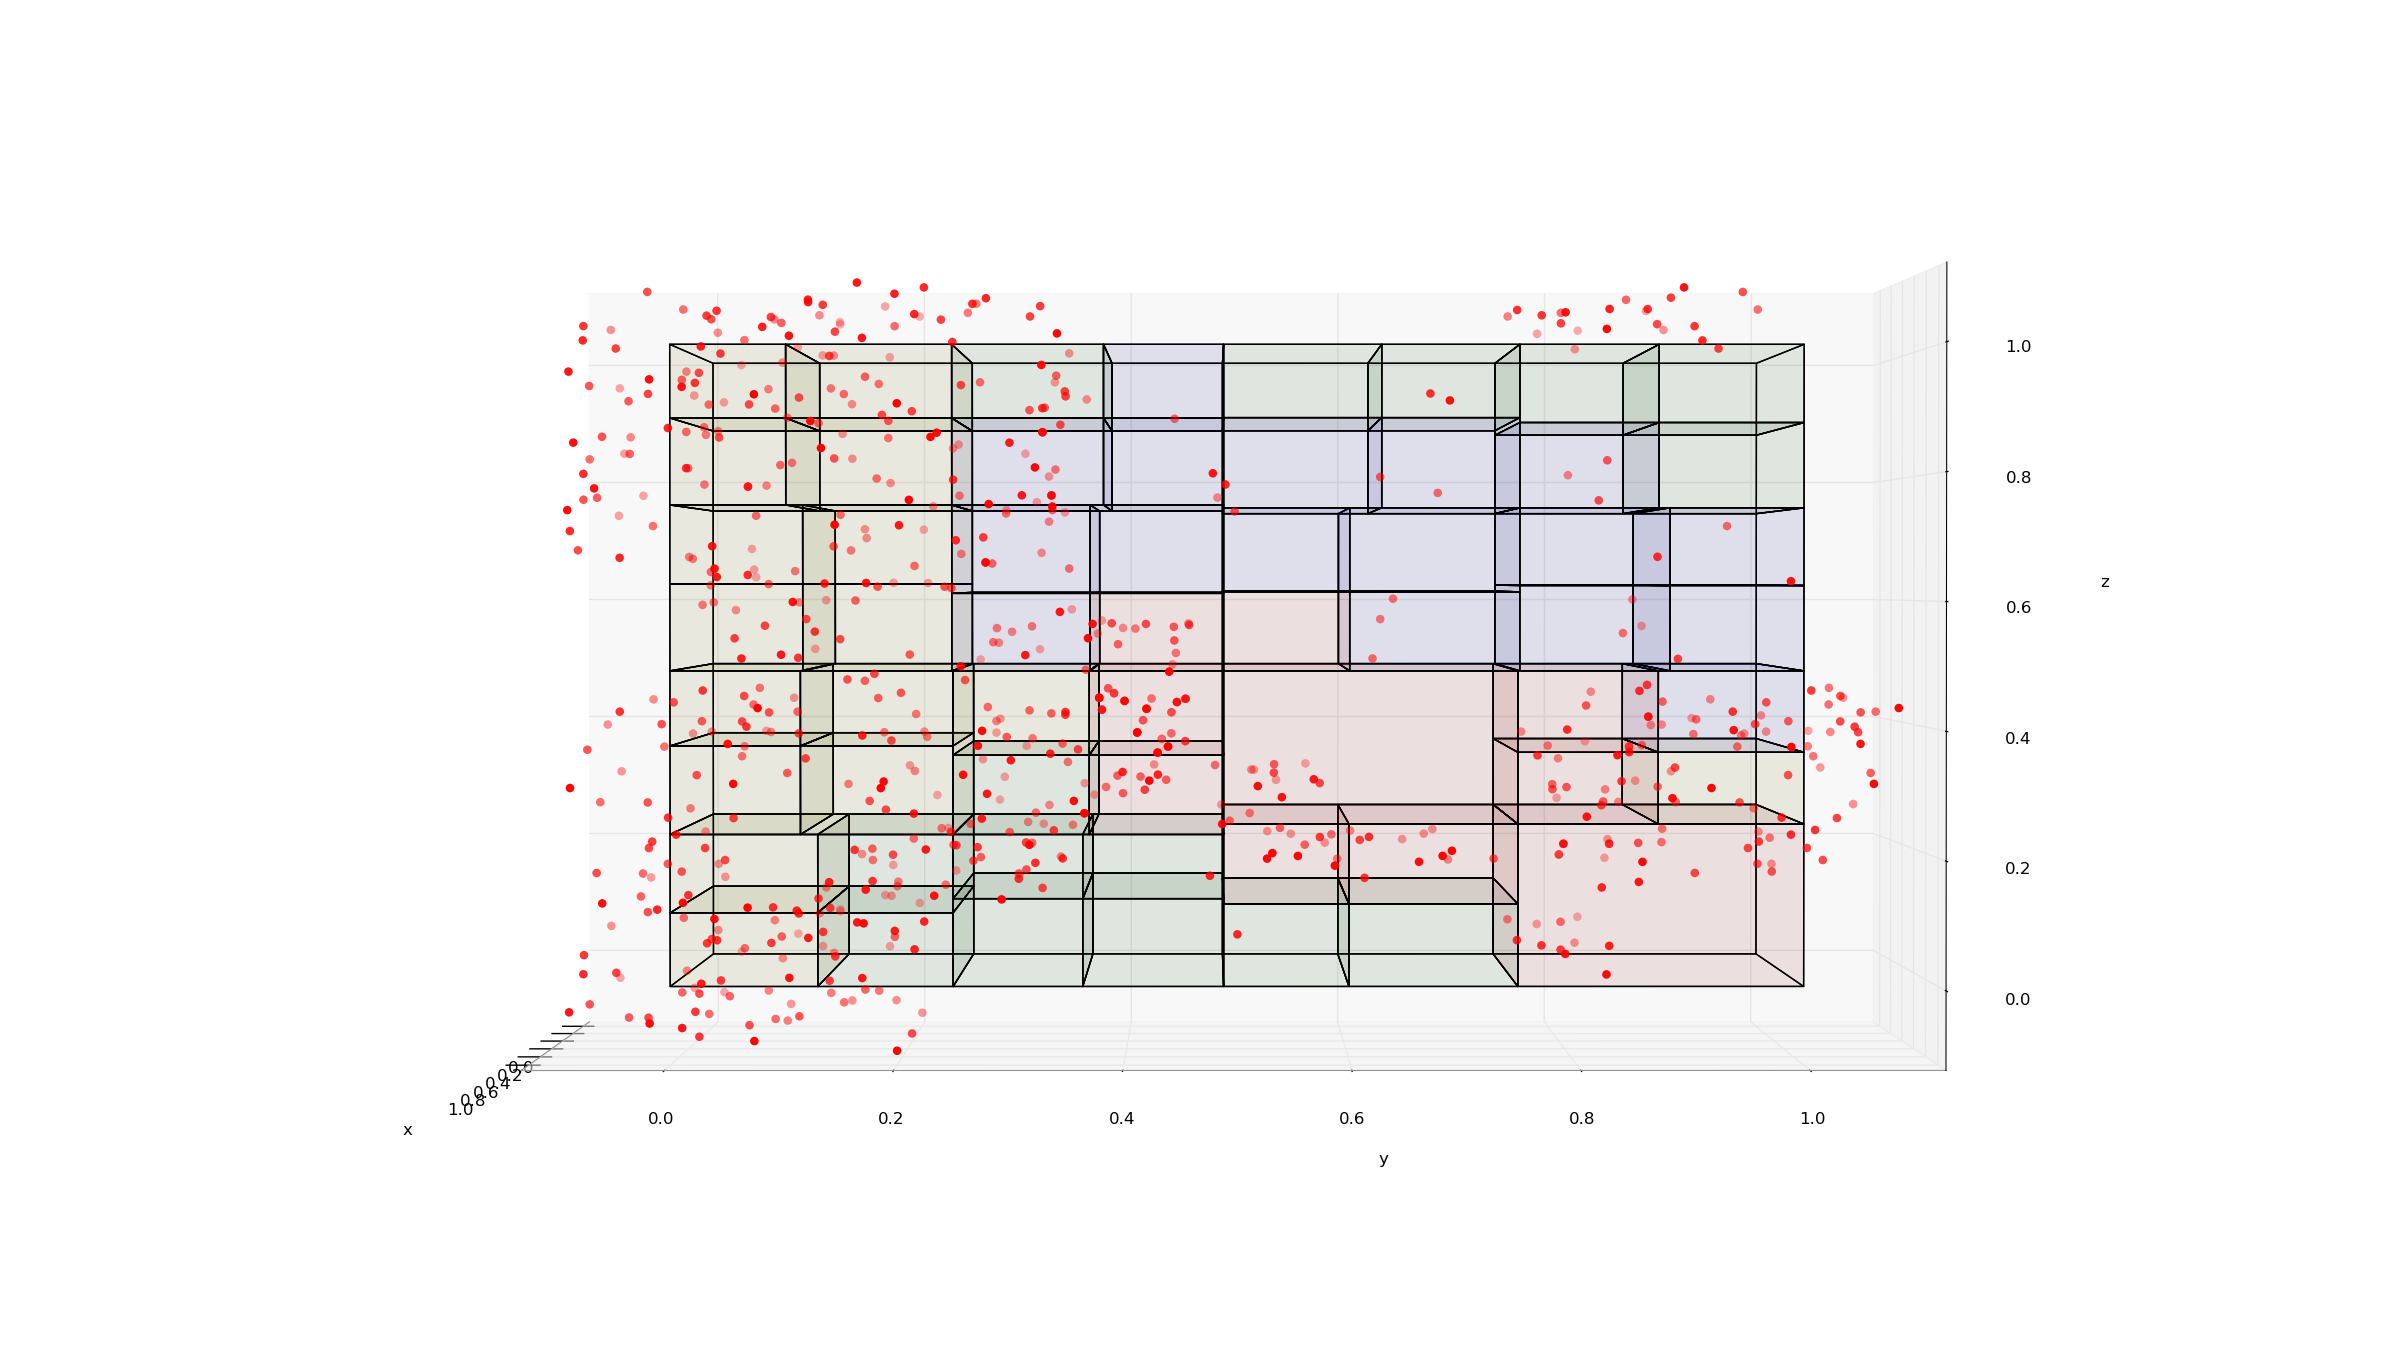
\includegraphics[width=0.5\columnwidth]{pics/ppm_decomp}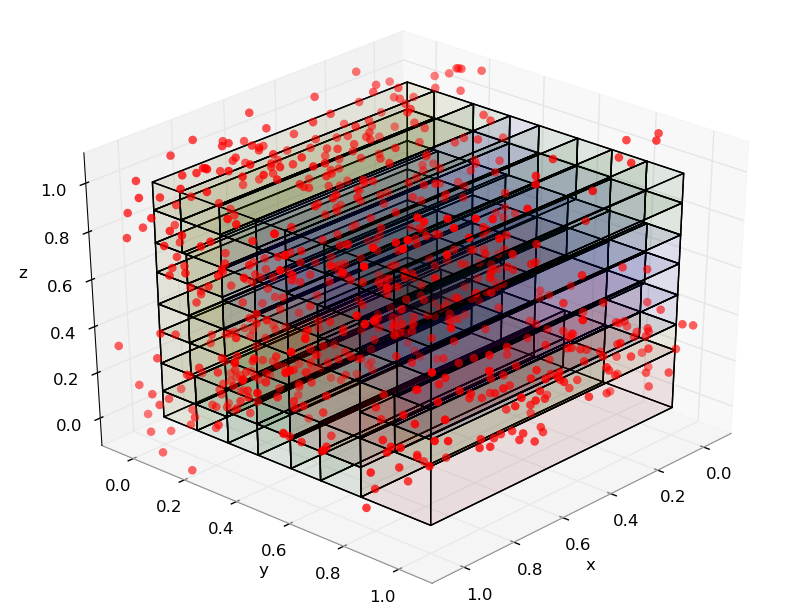
\includegraphics[width=0.5\columnwidth]{pics/ppm_slab_decomp}

\caption{Example of slab domain decomposition based on particles\label{fig:slab_domain_decomp}}


\end{figure}



\subsection{Distinguish: Mesh / Field }

Meshes are created on subdomains. Therefore the subs extents must
be compatible with the mesh spacing in all spatial dimensions. This
means: the sub extent must be an integer multiple of the mesh spacing. 

User defines the number of mesh points (not cells!) of the global
mesh in all dimensions. The mesh spacing is then computed internally
from this number and the extent of the physical domain. There is always
a grid point placed right ON the boundary of the computational domain
(PUT A SKETCH HERE). 

Due to above-mentioned compatibility contraint, sub boundary faces
always collocate with mesh planes (lines in 2D). The mesh points ON
these planes belon to BOTH subs. This seemingly unneccessary duplication
of points is motivated by: 
\begin{enumerate}
\item provide a convergence criterion for the Multigrid 
\item in the case of periodic outer B.C. the situation is consistent (the
points coincide around the boundary. 
\item internal boundaries (between subs) and external ones (comput. domain)
can be treated the same and the solvers do not need to care about
where there subs are locates. 
\item M'4 remeshing needs a ghostlayer of size 1 on all sides. Otherwise
it would have needed size 1 on one side and 2 on the other. Asymmetric
ghost layers are a pain for the mapping functions. 
\end{enumerate}
Circumvent by: not computing the same point twice (or compute and
use as convergence detection). 

When doing a field or field ghost mapping, the values on the duplicated
mesh nodes are actually exchanged (replaced with the value on the
same mesh point on the other sub or added for the ghost put). This
always applies to all internal sub boundaries and in case of periodic
boundary conditions also for the mesh points right on the boundary
of the computational domain. (of course only in periodic directions).
This whole paragraph is maybe too messy and there should be a better
way to describe this. Maybe also add a figure.


\subsection{Particle Based }

The domain decomposition can be driven by the positions of the particles.
In that case PPM creates subdomains such that each of them contains
a similar number of particles. To better equidistribute the computational
load between the processors, a cost-per-particle can be given as an
input argument. PPM will then adjust the sizes of the subdomains such
that the cost is equidistributed.

\begin{lstlisting}[language=Fortran]
CALL ppm_mktopo(topoid,xp,np,decomp,assig,min_phys,max_phys,bcdef,ghostsize,cost,info)
\end{lstlisting}



\subsection{Field Based }

If a mesh is provided in the argument list, then the subdomains are
created such that their boundaries coincide with the grid lines of
the mesh. This is necessary if one wants to use PPM's data structure
for meshes. 

\begin{lstlisting}[language=Fortran]
CALL ppm_mktopo(topoid,meshid,xp,np,decomp,assig,min_phys,max_phys,bcdef,ghostsize,cost,istart,ndata,nm,info)
\end{lstlisting}



\subsubsection{Different decompositions}

the fifth parameter of \texttt{the ppm\_mktopo} subroutine provides
a variety of methods for domain decomposition, which are listed below
: 
\begin{itemize}
\item ppm\_param\_decomp\_pruned\_cell 
\item ppm\_param\_decomp\_tree 
\item ppm\_param\_decomp\_bisection 
\item ppm\_param\_decomp\_xpencil 
\item ppm\_param\_decomp\_ypencil 
\item ppm\_param\_decomp\_zpencil 
\item ppm\_param\_decomp\_xy\_slab 
\item ppm\_param\_decomp\_xz\_slab 
\item ppm\_param\_decomp\_yz\_slab 
\item ppm\_param\_decomp\_cuboid 
\item ppm\_param\_decomp\_user\_defined 
\end{itemize}

\subsubsection{Load balancing}


\section{Meshes}

Example: defining a topology containing a mesh and allocating a field
array with the right size (accounting for ghost layers).

\begin{lstlisting}[language=Fortran,numbers=left]
CALL ppm_mktopo(topoid,meshid,xp,np,decomp,assig,min_phys,max_phys,bcdef,ghostsize,cost,istart,ndata,nm,info)
ALLOCATE(field_wp(nspec,(1-ghostsize(1)):(ndata(1,1)+ghostsize(1)),(1-ghostsize(2)):(ndata(2,1)+ghostsize(2)),1))
\end{lstlisting}



\section{Mapping between particles and processors}

Redistributes particles to their corresponding processor (as defined
by the topology).


\subsection{Global mapping}

All-to-all communication.

\begin{lstlisting}[breaklines=true,language=Fortran]
CALL ppm_map_part_global(topoid,xp,Npart_old,info) ! positions         
CALL ppm_map_part_push(wp1,Npart_old,info) ! strengths         
CALL ppm_map_part_push(wp2,dim2,Npart_old,info) ! vector property         
CALL ppm_map_part_send(Npart_old,Npart_new,info) ! send         
CALL ppm_map_part_pop(wp2,dim2,Npart_old,Npart_new,info)         
CALL ppm_map_part_pop(wp1,Npart_old,Npart_new,info)          
CALL ppm_map_part_pop(xp,ndim,Npart_old,Npart_new,info)
\end{lstlisting}



\subsection{Partial mapping}

Communication restricted to neighboring processors. This is much faster
and is generally used to update the mappings when particles have moved
(this assumes that no particle has moved further than the width of
one subdomain).

\begin{lstlisting}[breaklines=true,language=Fortran]
CALL ppm_map_part_partial(topoid,xp,Npart_old,info) ! positions         
CALL ppm_map_part_push(wp1,Npart_old,info) ! strengths         
CALL ppm_map_part_push(wp2,dim2,Npart_old,info) ! vector property         
CALL ppm_map_part_send(Npart_old,Npart_new,info) ! send         
CALL ppm_map_part_pop(wp2,dim2,Npart_old,Npart_new,info)         
CALL ppm_map_part_pop(wp1,Npart_old,Npart_new,info)          
CALL ppm_map_part_pop(xp,ndim,Npart_old,Npart_new,info)
\end{lstlisting}



\section{Ghost layers - mappings}


\subsection{Description of ghost layers}


\subsection{Communications to and from ghost layers}

Explain how the data in the ghost layers is communicated across processors


\subsection{Ghost mappings for meshes}

\begin{lstlisting}[breaklines=true,language=Fortran]
!-------------------------------------------------------------
!update the ghosts of velocity and vorticity fields   
!-------------------------------------------------------------
CALL ppm_map_field_ghost_get(topoid,mesh_id,ghostsize,info)   
CALL ppm_map_field_push(topoid,mesh_id,field_vorticity,vdime,info)   
CALL ppm_map_field_push(topoid,mesh_id,field_velocity,vdime,info)   
CALL ppm_map_field_send(info)   
CALL ppm_map_field_pop(topoid,mesh_id,field_velocity,vdime,ghostsize,info)   
CALL ppm_map_field_pop(topoid,mesh_id,field_vorticity,vdime,ghostsize,info)
\end{lstlisting}



\subsection{Ghost mappings for particles}

\begin{lstlisting}[breaklines=true,language=Fortran]
!-------------------------------------------------------------
!update the properties wp1 and wp2 on the ghost particles
!-------------------------------------------------------------
CALL ppm_map_part_ghost_get(topoid,xp,ndim,Npart,isymm,cutoff,info) 
CALL ppm_map_part_push(wp1,Npart,info) 
CALL ppm_map_part_push(wp2,Npart,info) 
CALL ppm_map_part_send(Npart,Mpart,info) 
CALL ppm_map_part_pop(wp2,Npart,Mpart,info) 
CALL ppm_map_part_pop(wp1,Npart,Mpart,info) 
CALL ppm_map_part_pop(xp,ndim,Npart,Mpart,info)
\end{lstlisting}



\subsection{Other routines}

ppm\_map\_type\_isactive: query the current map type.

This can be used to check if we are currently mapping ghost\_gets
and can skip the the ghost\_get itself only issuing push/send/pops.
Useful when particles have not moved.


\section{Neighbour lists}


\subsection{Homogeneous neighbour lists}

Here the variable cutoff is a real. All the particles have the same
cutoff radius.

\begin{lstlisting}[breaklines=true,language=Fortran]
CALL ppm_neighlist_vlist(topoid,xp,Mpart,cutoff,skin,symmetry,vlist,nvlist,info)
\end{lstlisting}



\subsection{Inhomoneneous neigbour lists (multiresolution)}

Here the variable cutoff is an array (every particle has its own cutoff
radius)

\begin{lstlisting}[breaklines=true,language=Fortran]
CALL ppm_inl_vlist(topo_id,xp,Npart,Mpart,cutoff,skin,symmetry,ghostlayer,info,vlist,nvlist) 
\end{lstlisting}



\subsection{Cross-set inhomoneneous neigbour lists (multiresolution)}

Construct the list of neighbours of one set of particles (blue particles)
for each particle of another set (red particles). Here the variable
cutoff is an array (every particle has its own cutoff radius)

\begin{lstlisting}[breaklines=true,language=Fortran]
CALL ppm_xset_inl_vlist(topo_id,xp_red,Np_red,Mp_red,xp_blue,Np_blue,Mp_blue,cutoff_blue,skin,ghostlayer,info,vlist,nvlist) 
\end{lstlisting}



\section{Boundary conditions}

The topology data structure contains information about the boundaries
of each subdomain. Each subdomain has 4 or 6 boundaries (in 2d and
3d, respectively), which can be independently internal or external.
TODO: describe this in more detail? (see source code of the data structure
for more).

Example: enforcing a Dirichlet boundary condition on a field.

\begin{lstlisting}[breaklines=true,language=Fortran]
!Boundary condition on phi     
dirichlet_value = -1._MK
DO isub=1,topo%nsublist         
	isubl = topo%isublist(isub)
    !Check whether this subdomain has external boundaries         
	! if so, applies dirichlet boundary condition      
	
	!west boundary?
	IF (topo%subs_bc(1,isubl) .NE. 0) THEN             
		field_wp(1,1,:,:,isub) = dirichlet_value         
	ENDIF
	!east boundary?         
	IF (topo%subs_bc(2,isubl) .NE. 0) THEN             
		field_wp(1,ndata(1,isubl),:,:,isub) = dirichlet_value         
	ENDIF
	!south boundary?
	IF (topo%subs_bc(3,isubl) .NE. 0) THEN             
		field_wp(1,:,1,:,isub) = dirichlet_value         
	ENDIF
	!north boundary?         
	IF (topo%subs_bc(4,isubl) .NE. 0) THEN             
		field_wp(1,:,ndata(2,isubl),:,isub) = dirichlet_value         
	ENDIF
	!bottom boundary?         
	IF (topo%subs_bc(5,isubl) .NE. 0) THEN             
		field_wp(1,:,:,1,isub) = dirichlet_value         
	ENDIF
	!top boundary?         
	IF (topo%subs_bc(6,isubl) .NE. 0) THEN             
		field_wp(1,:,:,ndata(3,isubl),isub) = dirichlet_value         
	ENDIF
END DO 
\end{lstlisting}



\chapter{Numerical methods}


\section{ODE solver}

\textbf{NOTE: this section's tutorial uses the old PPM datastructure
and should be updated to the new one.}

Example: we want to integrate 
\begin{equation}
\frac{du_{p}}{dt}=-\lambda u_{p}
\end{equation}
 on the particles using the 4th order Runge-Kutta of the ODE suite.

We'll assume that we have \lstinline!np! particles with positions
\lstinline!xp! and values \lstinline!up! already allocated and initialized. 


\subsection{Local variables}

\begin{lstlisting}[language=Fortran]
REAL(mk), DIMENSION(:,:), POINTER :: dup ! du/dt on particles 
REAL(mk), DIMENSION(:,:), POINTER :: bfr ! storage space for the stages 
REAL(mk), DIMENSION(4) :: time ! time things 
INTEGER :: istage ! stage counter 
INTEGER :: nstages ! number of stages 
INTEGER :: bfrsz ! size of the buffer "bfr" 
INTEGER :: scheme ! which scheme to use 
INTEGER :: odeid ! handle on the solver 
LOGICAL :: adapt ! use adaptive time step 
INTEGER :: lda ! leading dimension of our mode 
INTEGER, EXTERNAL :: MyRHS ! your implementation of the RHS
\end{lstlisting}



\subsection{Initialize the ODE Suite}

\begin{lstlisting}[language=Fortran]
!------------------------------------------------
! Initialize the Ode solver 
!------------------------------------------------
CALL ppm_ode_init (info)
\end{lstlisting}



\subsection{Create Mode}

\begin{lstlisting}[breaklines=true,language=Fortran]
scheme = PPM_PARAM_ODE_SCHEME_RK4 ! we want the 4th order RK scheme 
odeid = -1 ! let the PPM choose an ID for us 
adapt = .FALSE.! don't need adaptive time stepping 
lda = 2 
!----------------------------------------------- 
! Create the mode 
!-----------------------------------------------
CALL ppm_ode_create_ode(odeid, bfrsz, nstages, scheme, scheme, adapt, info)
\end{lstlisting}



\subsection{Allocate space for the stages}

\begin{lstlisting}[language=Fortran]
ALLOCATE(bfr(bfrsz*lda,np))
\end{lstlisting}



\subsection{Set the time}

\begin{lstlisting}[language=Fortran]
dt = 0.1 
time(1) = 0.0 
! set the start time 
time(2) = 1.0 
! set the end time 
time(3) = 0.0 
! set the current time 
time(4) = dt 
! set the time step size
\end{lstlisting}



\subsection{Start the ode solver}

Once all the modes have been created, start the ode solver.

\begin{lstlisting}[language=Fortran]
CALL ppm_ode_start(info)
\end{lstlisting}



\subsection{Start the time integration}

\begin{lstlisting}[breaklines=true,language=Fortran]
DO WHILE(.NOT.ppm_ode_alldone(info))
DO istage=1,nstages
CALL ppm_ode_step(odeid, xp, up, dup, lda, np, & & bfr, istage, time, MyRHS, info=info)
!-- say particles move, then we need to map after each stage 
maptype = ppm_param_map_partial 
CALL ppm_map_part(xp,3,np,mpart,topo_id,maptype,info) 
maptype = ppm_param_map_push 
CALL ppm_map_part(up,lda,np,mpart,topo_id,maptype,info) 
CALL ppm_map_part(dup,lda,np,mpart,topo_id,maptype,info) 
!-- now have the ode suite map the stages 
CALL ppm_ode_map_push(odeid,bfr,lda,np,mpart,info) 
!-- send maptype = ppm_param_map_send 
CALL ppm_map_part(dup,lda,np,mpart,topo_id,maptype,info) 
!-- pop in the reverse order 
CALL ppm_ode_map_pop(odeid,bfr,lda,np,mpart,info) 
maptype = ppm_param_map_pop 
CALL ppm_map_part(dup,lda,np,mpart,topo_id,maptype,info) 
CALL ppm_map_part(up,lda,np,mpart,topo_id,maptype,info) 
CALL ppm_map_part(xp,3,np,mpart,topo_id,maptype,info) 
END DO
END DO
CALL ppm_ode_finalize(info)
\end{lstlisting}



\subsection{The right-hand side}

A possible implementation of the function MyRHS

\begin{lstlisting}[language=Fortran]
FUNCTION MyRHS(vxp, vup, vdup, vdime, vnp, rpack, ipack, lpack, info) 
USE myGlobalData
!-- Arguments 
INTEGER, INTENT(in) :: vdime, vnp 
REAL(mk),DIMENSION(:,:),POINTER :: vxp, vup, vdup 
REAL(MK),DIMENSION(:,:), POINTER,OPTIONAL :: rpack 
INTEGER, DIMENSION(:,:), POINTER,OPTIONAL :: ipack 
LOGICAL, DIMENSION(:,:), POINTER,OPTIONAL :: lpack 
INTEGER, INTENT(inout) :: info INTEGER :: MyRHS
!-- Local variables 
INTEGER :: p
!-- Compute the right-hand side 
! assuming the parameter REAL(mk), DIMENSION(2) :: lambda 
! is specified in the module myGlobalData 
DO p=1,vnp 
	dup(1,p) = -lambda(1) * up(1,p) dup(2,p) = -lambda(2) * up(2,p) 
END DO
!-- bogus return value MyRHS = 123456 
RETURN 
END FUNCTION MyRHS 
\end{lstlisting}



\section{Particle remeshing}


\subsection{mesh-to-particle interpolation (ppm\_interp\_m2p) }

\begin{lstlisting}[language=Fortran]
CALL ppm_interp_m2p(topoid,meshid,xp,np,wp,1,kernel,ghostsize,field_wp,info)
\end{lstlisting}


NOTE: there is no need to update the ghost layers (for field\_wp)
prior to this call. 


\subsection{particle-to-mesh interpolation (ppm\_interp\_p2m)}

\begin{lstlisting}[language=Fortran]
CALL ppm_interp_p2m(topoid,meshid,xp,np,wp,1,kernel,ghostsize,field_wp,info)
\end{lstlisting}


NOTE: there is no need to update the ghost particles (for xp) prior
to this call. ppm\_interp\_p2m uses the ghost\_put mapping routines
internally. 


\section{Particle--particle interactions}


\chapter{I/O and visualisation}


\section{Parallel I/O}

ppm\_io, ASCII, binary, etc...

Not many formats are supported {}``out-of-the-box'', but some are
under development and should be available soon (e.g. VTK, HDF5).


\section{Tools}

{[}Under development{]} Visualisation of the domain decomposition,
positions of the particles (ghost and/or real particles) and of the
ghost layers (e.g. see figure \ref{fig:slab_domain_decomp}).


\chapter{Data structure for particles}

In the {}``dcops'' branch of PPM, there is a derived type for particles
(ppm\_t\_particles) and a collection of routines that perform some
standard/basic operations on these particles. The aim is to make it
easier to write clients for the library, without having to compromise
on flexibility nor on computational efficiency.

The different fields of the data structure are presented below. Note
that most of these fields can remain empty (nullified pointers) such
that the memory overhead is negligible. Some of the subroutines that
can be used with this data structure are explained briefly. The main
idea is that they check a bunch of pre-conditions and exit with an
error message if any of these conditions is not fulfilled. Otherwise,
it performs a task (usually passing data pointers to one or several
low-level PPM subroutines), updates some book keeping variables in
the data structure (post-conditions) and exits.


\section{Data}
\begin{itemize}
\item xp: array of positions
\item wpi: array of pointers to integer properties
\item wps: array of pointers to scalar properties
\item wpv: array of pointers to vector properties
\item ops: container for DC operators
\item nvlist: number of neighbours
\item vlist: Verlet lists
\end{itemize}

\subsection{Sizes}
\begin{itemize}
\item Npart: local number of real particles
\item Mpart: local number of real+ghosts particles
\item nwpi: number of integer properties
\item nwps: number of scalar properties
\item nwpv: number of vector properties
\end{itemize}

\subsection{Properties}

The pointers in wpi, wps and wpv point to derived types that hold
one property that is being carried by the particles. These derived
types (ideally, there should be one for each data type that PPM supports....)
contain
\begin{itemize}
\item vec: array that contains the actual data (it is 1d for scalar properties
and 2d for vector ones)
\item name: the name of that property (optional, but useful for keeping
track of what is what)
\item has\_ghosts: boolean that is true only when the ghost values for this
property are up-to-date
\item is\_mapped: boolean that is true only when there is a one-to-one mapping
between particles and this property
\item map\_parts: if true (default), then the mapping between this property
and the particles is kept over time (e.g. during a partial mapping
or after interpolation)
\item map\_ghosts: if true (default), then the ghost values for this property
are kept up-to-date (whenever a ghost mapping is called). Otherwise,
this property is not communicated.
\end{itemize}

\section{Variables and parameters}


\subsection{Neighbour lists}
\begin{itemize}
\item cutoff
\item skin
\item isymm
\end{itemize}

\subsection{Adaptive particles}
\begin{itemize}
\item rcp\_id: index where cutoff radii are stored
\item D\_id: index where preferred distance D is stored
\item Dtilde\_id: index where local monitor function is stored
\item adapt\_wpid: index where the field on which the monitor function depends
is stored
\item G\_id: index where the anisotropy tensor is stored
\end{itemize}

\subsection{Level sets}
\begin{itemize}
\item level\_id: index where the level function is stored
\end{itemize}

\section{Logical flags/markers}
\begin{itemize}
\item areinside: all particles are inside the computational box
\item active\_topoid: active topology for the particles
\item has\_ghosts: ghost particles have been fetched
\item ontopology: all particles are on their corresponding processor (ie.
Npart is correct)
\item neighlists: neighbour lists are up-to-date
\item adaptive: particles are adaptive particles
\item anisotropic: particles are anisotropic
\item level\_set: particles carry a level set function
\end{itemize}

\section{Routines}

Here we assume that topoid refers to the id of a previously defined
topology and 

\begin{lstlisting}[language=Fortran]
TYPE(ppm_t_particles), POINTER :: Particles
\end{lstlisting}



\subsection{apply\_bc}

Apply boundary conditions (wraps particles around the domain for periodic
boundary conditions and deletes particles on the other side of freespace
boundary conditions. Does not include other types of BC, yet.)

\begin{lstlisting}
particles_apply_bc(Particles,topoid,info)
\end{lstlisting}



\subsection{mapping\_global}

\begin{lstlisting}
particles_mapping_global(Particles,topoid,info)
\end{lstlisting}



\subsection{mapping\_partial}

\begin{lstlisting}
particles_mapping_partial(Particles,topoid,info)
\end{lstlisting}



\subsection{mapping\_ghosts}

\begin{lstlisting}
particles_mapping_ghosts(Particles,topoid,info)
\end{lstlisting}

\begin{itemize}
\item Needs particles to be mapped onto the topology
\item Update ghosts for the properties with the flag {}``map\_ghosts''
set to true (default)
\end{itemize}

\subsection{Create a new property}

For a scalar property:

\begin{lstlisting}
particles_allocate_wps(Particles,prop_id,info,name=example)
\end{lstlisting}


for a vector property with 7 dimensions:

\begin{lstlisting}
particles_allocate_wpv(Particles,prop_id,7,info,name=example)
\end{lstlisting}


If prop\_id = 0, then a new id is returned. Otherwise, the existing
property with that id is overwritten.


\subsection{Compute neighbor lists}

\begin{lstlisting}
particles_neighlists(Particles,topoid,info)
\end{lstlisting}


Some options have not yet been implemented, e.g. symmetric interactions,
but that will not be difficult.


\subsection{Access to the variables}

To access the arrays where the data is stored, use

\begin{lstlisting}
wp => get_wps(Particles, prop_id)
\end{lstlisting}


where wp is a DIMENSION(:), POINTER (for a scalar property).

If this property is mapped onto the particles, this will return a
1D array of size (1:Npart). Else, it will print out an error and return
the NULL pointer. If the ghost values are also needed, use

\begin{lstlisting}
wp => get_wps(Particles, prop_id,with_ghosts=.TRUE.)
\end{lstlisting}


If the ghost values for this property are available, this will return
a 1D array of size (1:Mpart), else it will print out an error and
return the NULL pointer (which will probably crash the code a moment
later)

Once these arrays are no longer needed, it is strongly advised to
use the set\_wps functions (which do a bookkeeping job).

If the values have been changed:

\begin{lstlisting}
wp => set_wps(Particles, prop_id)
\end{lstlisting}


If the values have been changed but the ghost values have also been
changed (to their correct values, such that no further communication
is required), do:

\begin{lstlisting}
wp => set_wps(Particles, prop_id,ghosts_ok=.TRUE.)
\end{lstlisting}


If the values have been accessed but not changed, use:

\begin{lstlisting}
wp => set_wps(Particles, prop_id,read_only=.TRUE.)
\end{lstlisting}


There are corresponding functions for integer and vector properties
(get\_wpi, get\_wpv, ...) as well as for particles' positions:

\begin{lstlisting}
xp => get_xp(Particles)
\end{lstlisting}


Note that the following call

\begin{lstlisting}
xp => set_xp(Particles)
\end{lstlisting}


notifies the data structure that the particles have moved and updates
the state variables accordingly. For example, the particles are no
longer assumed to be within the bounds of the computational domain,
and the neighbor lists, the ghosts, the DC operators as now flagged
as being wrong. If the array xp has only be used for reading, one
should of course call

\begin{lstlisting}
xp => set_xp(Particles,read_only=.TRUE.)
\end{lstlisting}
instead.


\subsection{Manual override}

Some routines are here to do only a book keeping job. For example
if one wants to tell the library that the particles cutoffs have changed,
or that the particles have moved, or that their numbers have changed,
one can call 

updated\_cutoff, updated\_positions or updated\_nb\_part.

The internal variables will then be updated accordingly.


\section{Usage examples}

Let's solve a PDE of the form

\[
\frac{\partial w}{\partial t}=\frac{\partial^{2}w}{\partial x^{2}}-\frac{\partial w}{\partial y}+2\frac{\partial^{4}w}{\partial x\partial y^{3}}
\]
in a periodic box.

\begin{lstlisting}[breaklines=true,language=Fortran,numbers=left]
!Load necessary modules
USE ppm_module_particles
USE ppm_module_dcops
USE ppm_module_io_vtk

!Create a topology based on geometry (ie. define a simple box)
topoid = 0
call ppm_mktopo(topoid,decomp,assig,min_phys,max_phys,bcdef,cutoff,cost,info) 

!Initialize N particles inside the computational domain
call particles_initialize(Particles,np_global,info,ppm_param_part_init_cartesian,topoid)

!Move them around randomly by an amount of 0.15*h
allocate(disp(ndim,Particles%Npart)) 
call random_number(disp) 
disp=0.15_mk*Particles%h_avg*disp 
call particles_move(Particles,disp,info) 

!Put particles back into the box using periodic boundary conditions
call particles_apply_bc(Particles,topoid,info) 

!Define particles cutoff
Particles%cutoff = Particles%h_avg * 3.3_mk 

!Global mapping
call particles_mapping_global(Particles,topoid,info) 

!Allocate and initialize one property on these particles (using an external function f0_fun)
wp_id=0 
call particles_allocate_wps(Particles,wp_id,info) 
wp => Get_wps(Particles,wp_id); xp => Get_xp(Particles) 
FORALL(ip=1:Particles%Npart) wp(ip) = f0_fun(xp(1:ndim,ip),ndim) 
wp => Set_wps(Particles,wp_id); xp => Set_xp(Particles,read_only=.TRUE.) 

!Get ghost particles and update values for wp
call particles_mapping_ghosts(Particles,topoid,info)

!Compute neighbor lists
call particles_neighlists(Particles,topoid,info) 

!Allocate another field dwp
dwp_id=0 
call particles_allocate_wps(Particles,dwp_id,info)

!Define a DC operator to compute the RHS of the PDE
nterms=3 
allocate(degree(nterms*ndim),coeffs(nterms),order(nterms)) 
degree = (/2,0, 0,1, 1,3/) 
coeffs = (/1.0_mk, -1._mk, 2._mk/) 
order = (/2, 2, 2/)
eta_id = 0 
call particles_dcop_define(Particles,eta_id,coeffs,degree,order,nterms,info,name="my_rhs") 

!Compute the DC operator
call particles_dcop_compute(Particles,eta_id,info) 

DO WHILE (t < t_end)

	!Evaluate the DC operator using wp as input data and store the result in dwp
	call particles_dcop_apply(Particles,wp_id,dwp_id,eta_id,info) 

	!Update wp using a forward Euler scheme
	wp => Get_wps(Particles,wp_id)
	dwp => Get_wps(Particles,dwp_id)
	FORALL(ip=1:Particles%Npart)
		wp(ip) = wp(ip) + dt * dwp(ip)
	END FORALL
	wp => Set_wps(Particles,wp_id) 
	dwp => Set_wps(Particles,dwp_id,read_only=.TRUE.)

	!Update ghost values for wp (without recomputing the ghost mappings)
	call particles_mapping_ghosts(Particles,topoid,info)
ENDDO

!Printout the result in VTK format, to be read directly within e.g. Paraview
call ppm_vtk_particle_cloud('mydatafile',Particles,info)

!Free memory from this DC operator
call particles_dcop_free(Particles,eta_id,info) 

!Free memory from the particles
call ppm_alloc_particles(Particles,N,ppm_param_dealloc,info)
\end{lstlisting}



\chapter{Examples}

\bibliographystyle{plain}
\bibliography{tutorial}

\end{document}
